\hypertarget{RandomForest_8c}{
\section{RandomForest.c File Reference}
\label{RandomForest_8c}\index{RandomForest.c@{RandomForest.c}}
}
{\tt \#include \char`\"{}party.h\char`\"{}}\par


Include dependency graph for RandomForest.c:\nopagebreak
\begin{figure}[H]
\begin{center}
\leavevmode
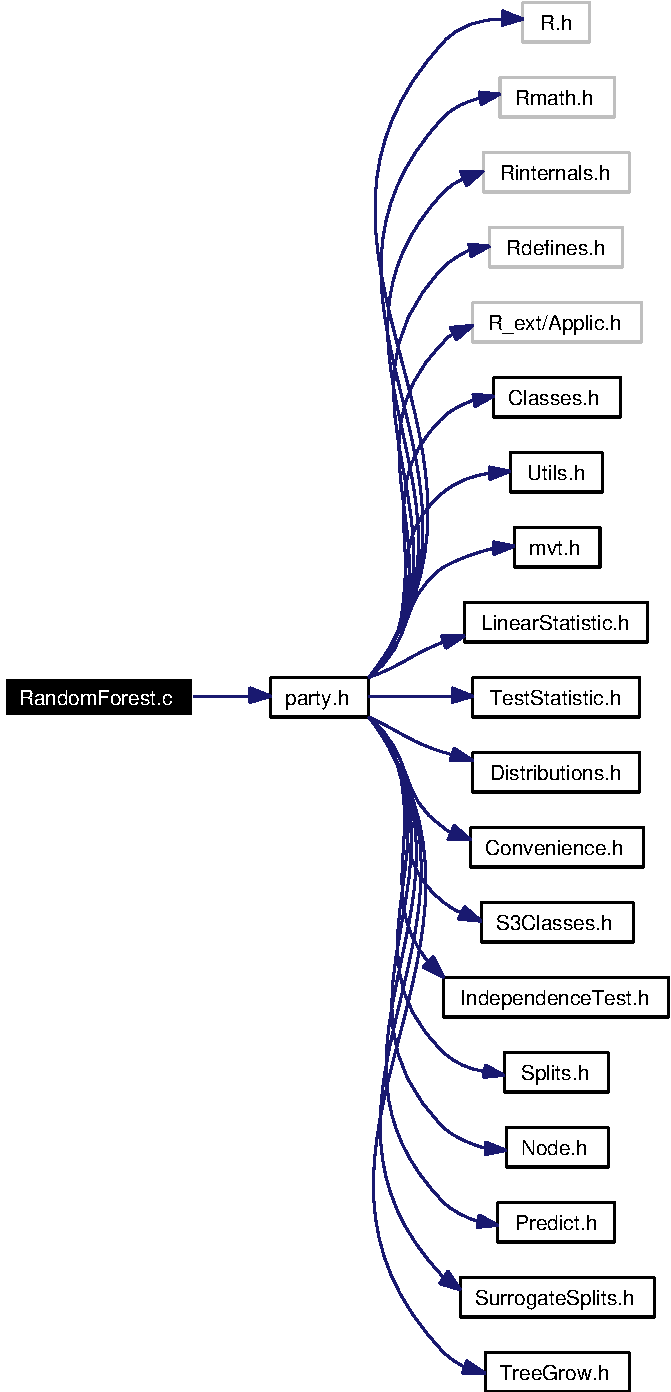
\includegraphics[width=420pt]{RandomForest_8c__incl}
\end{center}
\end{figure}
\subsection*{Functions}
\begin{CompactItemize}
\item 
SEXP \hyperlink{RandomForest_8c_4f54420cb561055a4e545f7e1359fb87}{R\_\-Ensemble} (SEXP learnsample, SEXP weights, SEXP bwhere, SEXP bweights, SEXP fitmem, SEXP controls)
\end{CompactItemize}


\subsection{Detailed Description}
Random forest with conditional inference trees

\begin{Desc}
\item[Author:]\end{Desc}
\begin{Desc}
\item[Author]hothorn \end{Desc}
\begin{Desc}
\item[Date:]\end{Desc}
\begin{Desc}
\item[Date]2007-07-23 10:09:38 +0200 (Mon, 23 Jul 2007) \end{Desc}


Definition in file \hyperlink{RandomForest_8c-source}{RandomForest.c}.

\subsection{Function Documentation}
\hypertarget{RandomForest_8c_4f54420cb561055a4e545f7e1359fb87}{
\index{RandomForest.c@{RandomForest.c}!R\_\-Ensemble@{R\_\-Ensemble}}
\index{R\_\-Ensemble@{R\_\-Ensemble}!RandomForest.c@{RandomForest.c}}
\subsubsection[{R\_\-Ensemble}]{\setlength{\rightskip}{0pt plus 5cm}SEXP R\_\-Ensemble (SEXP {\em learnsample}, \/  SEXP {\em weights}, \/  SEXP {\em bwhere}, \/  SEXP {\em bweights}, \/  SEXP {\em fitmem}, \/  SEXP {\em controls})}}
\label{RandomForest_8c_4f54420cb561055a4e545f7e1359fb87}


An experimental implementation of random forest like algorithms \par
 \begin{Desc}
\item[Parameters:]
\begin{description}
\item[{\em learnsample}]an object of class `LearningSample' \item[{\em weights}]a vector of case weights \item[{\em bwhere}]integer matrix (n x ntree) for terminal node numbers \item[{\em bweights}]double matrix (n x ntree) for bootstrap case weights \item[{\em fitmem}]an object of class `TreeFitMemory' \item[{\em controls}]an object of class `TreeControl' \end{description}
\end{Desc}


Definition at line 22 of file RandomForest.c.

References C\_\-init\_\-node(), C\_\-remove\_\-weights(), C\_\-SampleSplitting(), C\_\-TreeGrow(), get\_\-fraction(), get\_\-maxsurrogate(), get\_\-ninputs(), get\_\-nobs(), get\_\-ntree(), get\_\-predict\_\-trafo(), get\_\-replace(), get\_\-splitctrl(), ncol(), NODE\_\-LENGTH, PL2\_\-responsesSym, and S3get\_\-nodeweights().

Here is the call graph for this function:\nopagebreak
\begin{figure}[H]
\begin{center}
\leavevmode
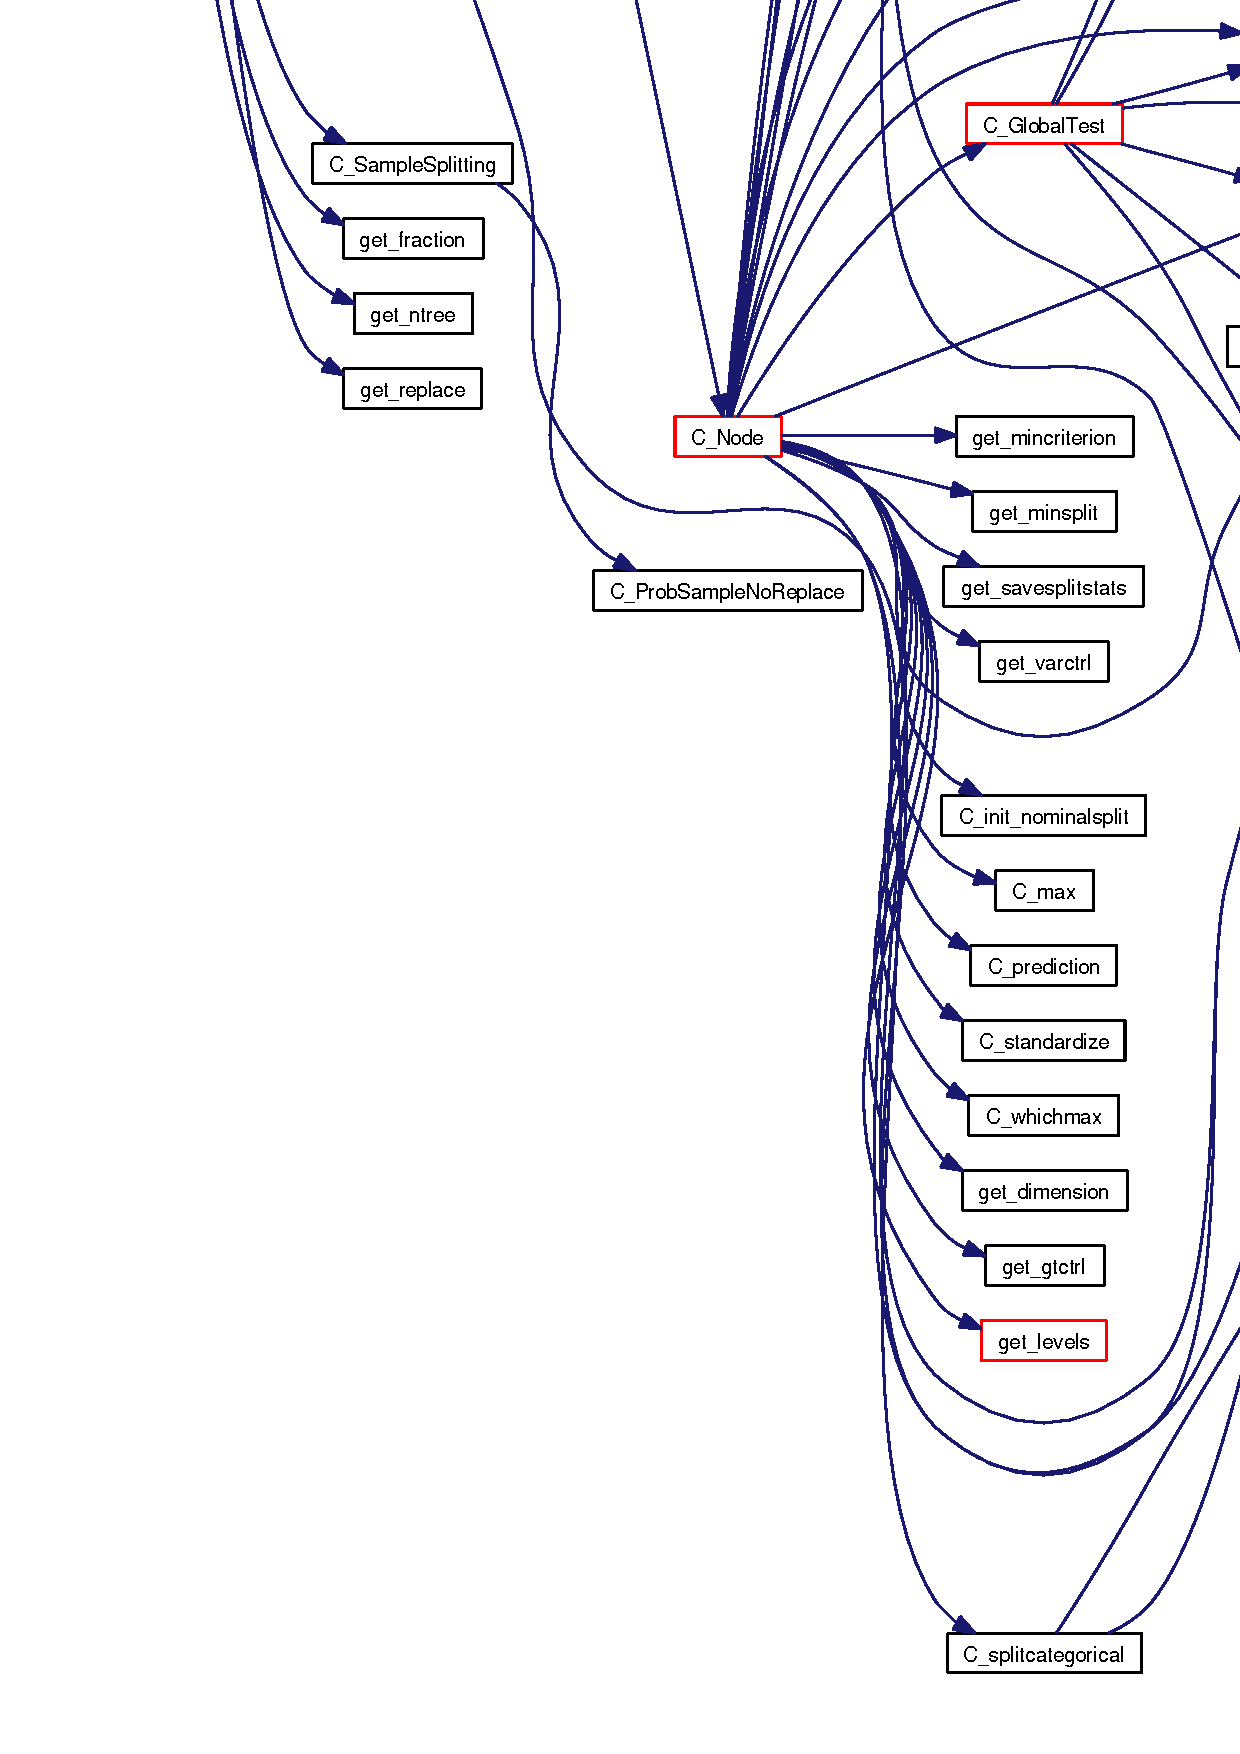
\includegraphics[width=386pt]{RandomForest_8c_4f54420cb561055a4e545f7e1359fb87_cgraph}
\end{center}
\end{figure}
